
If we measure an aspect of security before and after a change takes place, then we can quantify the impact that change had on security. If we test an aspect of cyber security at regular intervals, then we can determine the rate of change for that property over time. In order to sample security measurements at regular (approaching continuous) intervals, we assert that the test apparatus must be fully automated. The necessity of such automation is critical to evaluating security metrics in a repeatable and consistent way. 

\begin{figure}[ht]
\centering
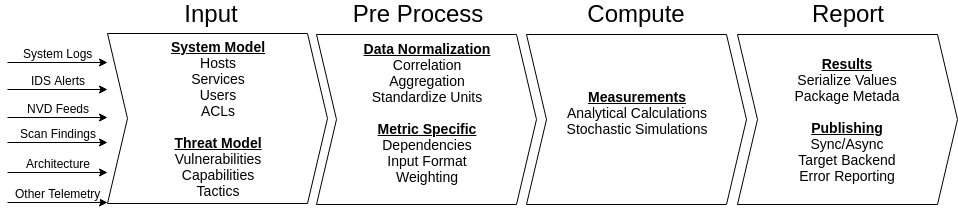
\includegraphics[width=\linewidth]{img/metric_calc_pipeline.png}
\caption{Generalized Metric Evaluation Pipeline}
\label{fig:automation:metric_pipeline}
\end{figure} 

In Figure \ref{fig:automation:metric_pipeline} we present a general four-stage pipeline for security metric processing based on our observations implementing a number of metrics from the literature. This abstraction encourages us to:
\begin{itemize}
\item Decouple the source of system information from the representation of that information. 
\item Decouple the actual calculation of the metric from the input model representation it is typically paired with in its publication. 
\item Decouple the calculation logic and supporting metadata from any assumptions about how that measured value will be used in the future. 
\end{itemize}

In doing so, it becomes possible to identify shared dependencies among metrics, enables a systematic examination of the characteristics and behaviours of each metric across a range of inputs, and supports more reusable and composeable components for a greater variety of deployment scenarios. The remainder of this section provides the considerations and details of each stage.

% The \textit{Pre Process} stage transforms the current knowledge base into a format suitable for the desired metric calculation. 

% \begin{figure}[ht]
% 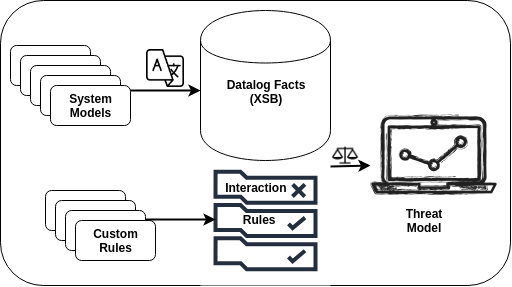
\includegraphics[width=.48\textwidth]{img/Ptah_archs.png}
% \caption{Preprocessing and Transformation Handlers (\textbf{PTaH})}
% \label{fig:automation:ptah_arch}
% \end{figure} 


% The \textit{Compute} stage implements the calculation of the security metric and takes the measurement of the current state. 

% Finally, the \textit{Reporting} stage handles the response logic needed to return the measured value and associated metadata appropriately. The remainder of this section provides the considerations and details of each stage.

% Development:
% \begin{enumerate}
% \item Vagrant and Ansible
% \item MulVal
% \begin{itemize}
% \item Multiple Rule Support
% \item Python-XSB interface
% \end{itemize}
% \item Collection and Publishing
% \end{enumerate}

% Evaluation:
% \begin{enumerate}
% \item Metric Pipeline
% \item Standard Metric Interface: SecMet
% \item Setup \& Preprocessing with Ptah
% \end{enumerate}

% Validation:
% \begin{enumerate}
% \item Properties of Valid Security Metrics
% \item A Validation Reference Set
% \item Validating Across Scales
% \item Validating Across Security Levels
% \end{enumerate}









